\section{AFL}

\begin{frame}{AFL}{Algorithme génétique}
  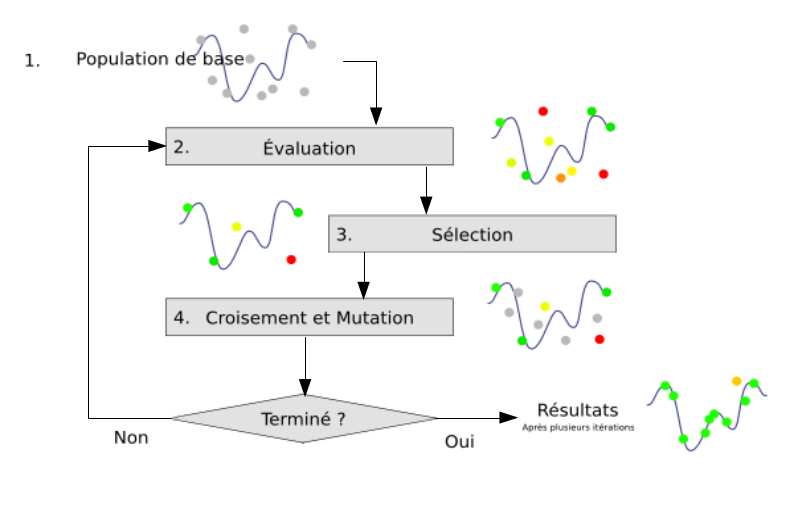
\includegraphics[width=\textwidth]{../medias/schema_genetique.png}
\end{frame}

\begin{frame}{AFL}{Mutations}
  \begin{quote}\Large
  "Designing the mutation engine for a new fuzzer has more to do with art than science"
  \end{quote}
  \begin{exampleblock}{Stratégies déterministes}
    \begin{itemize}
      \item{bit flip : \lstinline{1101 0010} devient \lstinline{1100 0010}} \pause
      \item{byte flip : \lstinline{0xdeadbeef} devient \lstinline{0xde52beef}} \pause
      \item{arithmétique simple : \lstinline{0xdeadbeef} devient \lstinline{0xdeafbeef}} \pause
      \item{constantes intéressantes : \lstinline{-1}, \lstinline{256}, \lstinline{INT_MAX}, ...} \pause
    \end{itemize}
  \end{exampleblock}
  \begin{exampleblock}{Stratégies aléatoires : empilement de plusieurs petites modifications}
    \begin{itemize}
      \item{unique bit flip} \pause
      \item{remplacement d'un byte aléatoirement ou par un autre intéressant} \pause
      \item{duplication de bloc via suppression ou insertion} \pause
      \item{memset de bloc}
    \end{itemize}
  \end{exampleblock}
\end{frame}

\begin{frame}{AFL}{Basic Block}
  \begin{figure}
    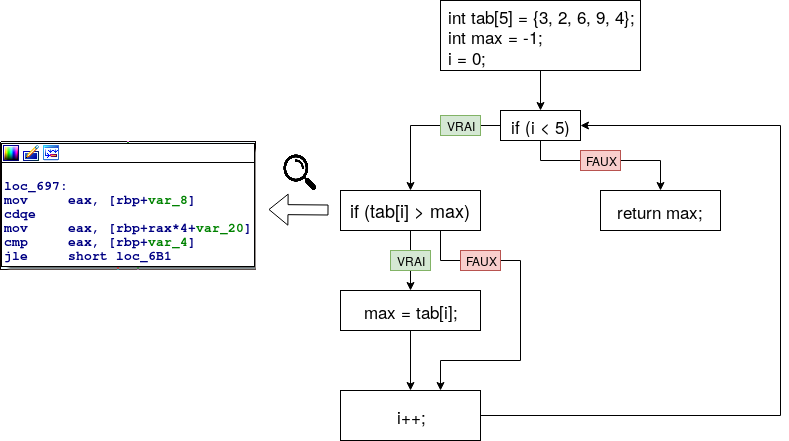
\includegraphics[width=1.0\textwidth]{../medias/BB_loupe.png}
  \end{figure}
\end{frame}

\begin{frame}[fragile]{AFL}{Instrumentation}
  {\Large \centerline{L'instrumentation est un bout de code rajouté par AFL au programme}}
  \begin{itemize}
    \item{Elle est faite au niveau de chaque basic bloc} \pause
  \end{itemize}

  \hspace{0.5cm}

  \begin{lstlisting}
    cur_location = <COMPILE_TIME_RANDOM>;
    shared_mem[cur_location ^ prev_location]++;
    prev_location = cur_location >> 1;
  \end{lstlisting}

  \pause
  \hspace{3.5cm}

  \begin{exampleblock}{Explications}
    \begin{itemize}
      \item{valeur aléatoire pour simplifier l'édition de lien} \pause
      \item{une case de \lstinline{shared_mem[]} correspond à une flèche du graphe précédent} \pause
      \item{shift pour différencier A $\rightarrow$ B de B $\rightarrow$ A, ainsi que A $\rightarrow$ A de B $\rightarrow$ B}
    \end{itemize}
  \end{exampleblock}
\end{frame}

\begin{frame}{AFL}{Transformation Basic Block}
  \begin{figure}
    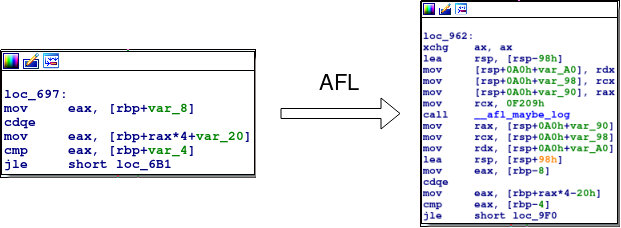
\includegraphics[width=1.0\textwidth]{../medias/block_to_afl.png}
  \end{figure}
\end{frame}

\begin{frame}{AFL}{Nouveaux comportements}
  \begin{columns}
    \begin{column}{0.5\textwidth}
      \begin{exampleblock}{Nouvelles transitions}
        \begin{itemize}
          \item{pas de comparaison des traces}
          \item{comparaison des transitions}
          \item{nouvelle transition intéressante}
        \end{itemize}
        \vspace{1.25ex}
      \end{exampleblock}
    \end{column}

    \begin{column}{0.5\textwidth}
      \begin{exampleblock}{Catégories}
        \begin{itemize}
          \item{\lstinline{shared_mem[]} rangé par catégories}
          \item{1, 2, 3, 4-7, 8-15, 16-31, 32-127, 128+}
          \item{changement de catégorie intéressant}
        \end{itemize}
      \end{exampleblock}
    \end{column}
  \end{columns}

  \pause
  \hspace{50.5cm}

  {\Large \centerline{Exemples}}

  \hspace{20.5cm}

  \begin{itemize}
    \item{\#1: A $\rightarrow$ B $\rightarrow$ B $\rightarrow$ A $\rightarrow$ C $\rightarrow$ D} \pause
    \item{\#2: A $\rightarrow$ B $\rightarrow$ A $\rightarrow$ B $\rightarrow$ A $\rightarrow$ C} \pause
    \item{\#3: A $\rightarrow$ B $\rightarrow$ C $\rightarrow$ D} \pause
    \item{\#4: A $\rightarrow$ B $\rightarrow$ A $\rightarrow$ B}
  \end{itemize}
\end{frame}

\begin{frame}{AFL}{Modèle "fork server" (1)}
  \begin{columns}[t]
    \begin{column}{0.49\textwidth}
      \begin{block}{"classique"}
        \begin{itemize}
        \item \lstinline{execve()}
          \begin{itemize}
          \item copie du programme en mémoire
          \item \lstinline{ld-linux.so} charge les librairies partagées
          \end{itemize}
        \item \lstinline{waitpid()}
        \item tout recommencer avec une autre entrée
        \end{itemize}
        \vspace{3.5ex}
      \end{block}
    \end{column}

    \begin{column}{0.49\textwidth}
      \begin{block}{"fork server"}
        \begin{itemize}
        \item \lstinline{execve()} "classique"
        \item programme cible instrumenté
          \begin{itemize}
          \item "pause" avant le \lstinline{main} du programme
          \item \lstinline{fork()} pour copier le processus
          \item \lstinline{waitpid()} pour surveiller les enfants
          \end{itemize}
        \item communication entre \lstinline{afl-fuzz} et programme parent avec un \lstinline{pipe}
        \end{itemize}
      \end{block}
    \end{column}
  \end{columns}
\end{frame}

\begin{frame}{AFL}{Modèle "fork server" (2)}
  \begin{columns}[t]
    \begin{column}{0.5\textwidth}
      \begin{center}
        \textbf{"classique"}
      \end{center}

      \bigskip
      \begin{figure}
        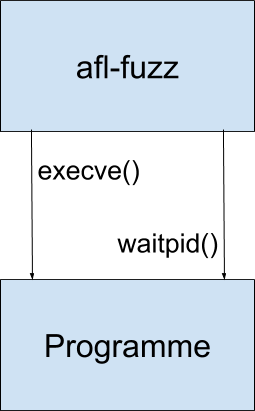
\includegraphics[width=.4\textwidth]{../medias/classique.png}
      \end{figure}
    \end{column}

    \begin{column}{0.5\textwidth}
      \begin{center}
        \textbf{"fork server"}
      \end{center}

      \begin{figure}
        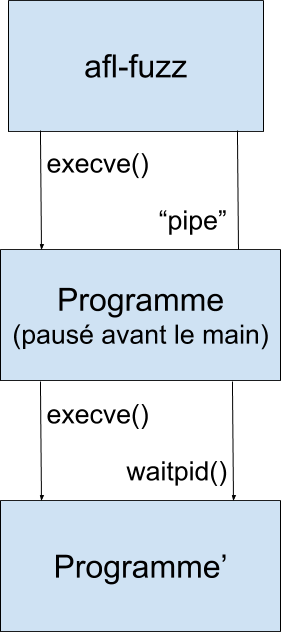
\includegraphics[width=.4\textwidth]{../medias/fork-server.png}
      \end{figure}
    \end{column}
  \end{columns}
\end{frame}
